\section{Hypothesis}

RJCB expects that the inference error is lowest for
parameter settings without multiple-births, for these settings, the
MBD model falls back to being a BD model, which is the standard speciation
model we assume to have generated the tree.

RJCB expects that the inference error is highest for
parameter settings with a higher percentage of multiple-births.
For these settings, the mismatch between the the speciation model that
generated the true tree (which is profoundly-MB MBD) is biggest with
the tree prior assumed to be generative (which is BD).

RJCB expects that an increased extinction rate
has a neutral effect on the error made, for runs with an equal percentage of MBness,
because extinction affects all species equally. 

RJCB expects that an increased number of taxa
has a negative effect on the variance of the errors made, as there
is more information available to base inference on.

RJCB expects that an increased extinction rate
increases the variance of the errors made,
due to the decrease of the number of taxa, reducing the amount of information
to base inference on.

RJCB expects that the distribution of nLTT statistics between
true trees and expected twin trees has the same shape
as the difference between the error between the true and twin phylogeny \richel{(see
Figure \ref{fig:nltt_as_proxy})}.
Due to this, the nLTT statistic can act as good shortcut
to arrive at the same conclusion.

\begin{figure}[!htbp]
  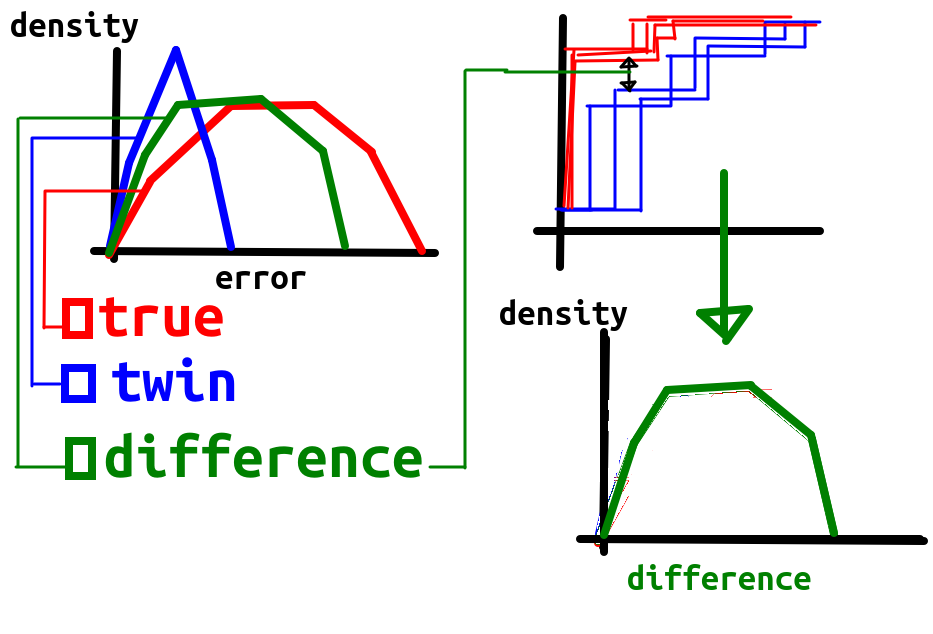
\includegraphics[width=\textwidth]{20191125_nltt_as_proxy.png}
  \caption{
    The nLTT statistic between true and twin tree is strongly related
    to the error between true and twin phylogeny.
  }
  \label{fig:nltt_as_proxy}
\end{figure}

